\documentclass[a4paper,10pt,twocolumn]{memoir}
\usepackage[utf8]{inputenc}
\usepackage[T1]{fontenc}
\usepackage{lmodern}
\usepackage{xcolor}
\usepackage{tikz}
\usepackage{geometry}
\usepackage{graphicx}
\usepackage{amsmath,amssymb}
\usepackage{hyperref}
\usepackage{tocloft}
\usepackage{parskip}
\usepackage{enumitem}
\usepackage{microtype}
\usepackage{fancyhdr}
\usepackage{lettrine}
\usepackage{pgfplots} 
\pgfplotsset{compat=1.18} 
\usepackage{caption}
\usepackage{titlesec}
\usepackage[most]{tcolorbox}
\usepackage{float}
\usepackage[titles]{tocloft}
\usepackage{eso-pic} % Add this to the preamble if not already present
\newcommand{\highlight}[1]{\textcolor{accent}{\textbf{#1}}}
\usepackage{multicol} % for two-column TOC
\tcbuselibrary{listings, skins, breakable}  % optional enhancements
\usetikzlibrary{shapes.geometric, arrows, positioning}

%Quote package define
\usepackage{framed}
\definecolor{shadecolor}{RGB}{240,240,240}
\newenvironment{magquote}
  {\begin{shaded*}\itshape\small}
  {\end{shaded*}}

% Page geometry
\geometry{
  a4paper,
  left=15mm,
  right=15mm,
  top=20mm,
  bottom=15mm,  % Reduced bottom margin
  columnsep=8mm
}

% Color palette
\definecolor{primary}{RGB}{30, 50, 100}
\definecolor{accent}{RGB}{200, 80, 0}
\definecolor{light}{RGB}{245, 245, 248}
\definecolor{dark}{RGB}{40, 40, 45}
\definecolor{gray}{RGB}{120,120,120}  % Defined gray color

% Typography
\renewcommand{\familydefault}{\sfdefault}
\setlength{\parindent}{0pt}
\setlength{\parskip}{0.7em}  % Slightly tighter paragraph spacing
\linespread{1.05}
\frenchspacing

% Header/Footer
\pagestyle{fancy}
\fancyhf{}
\fancyhead[L]{\footnotesize\scshape\color{primary}The Aevum}
\fancyhead[R]{\footnotesize\color{primary}June 2025}
\fancyfoot[C]{\thepage}
\renewcommand{\headrulewidth}{0.4pt}
\renewcommand{\headrule}{\hbox to\headwidth{\color{accent}\leaders\hrule height \headrulewidth\hfill}}

% Article command
\newcommand{\article}[3]{
  \section*{#1}
  \addcontentsline{toc}{section}{#1}
  \begin{center}
    \color{dark}\normalsize\textbf{#2}\\
    \small\color{gray}#3
  \end{center}
  \vspace{-0.8em}  % Tighter spacing
}
%Udoy er command
\newcommand{\highlight}[1]{\textcolor{accent}{\textbf{#1}}}


% Contributor command
\newcommand{\contributor}[4]{%
  \vspace{0.3em}
  \begin{tcolorbox}[
    colback=light,
    colframe=primary,
    boxrule=0.5pt,
    arc=2mm,
    left=3mm,
    right=3mm,
    top=2mm,
    bottom=2mm
  ]
    \textbf{\normalsize #1}\\
    {\footnotesize Roll: #2 \quad Reg: #3}\\
    {\footnotesize\color{gray}\itshape Role: #4}
  \end{tcolorbox}
}


\begin{document}

% Front Cover
\begin{titlingpage}
\AddToShipoutPictureBG*{%
  \AtPageLowerLeft{%
    \includegraphics[width=\paperwidth, height=\paperheight]{cover.png}
   
  }
}
 \null
\end{titlingpage}

% Prologue and Table of Contents

\begin{titlingpage}
\thispagestyle{empty}

% Single column layout for better control
\noindent
\begin{minipage}[t]{0.45\textwidth}
\section*{\centering\large\bfseries\color{primary}Prologue}
\vspace{0.5cm}
\tikz{\draw[accent, line width=0.8pt] (0,0) -- (\linewidth,0);}
\vspace{0.5cm}

\lettrine[lines=3]{I}{n} a world racing toward the future, where ideas spark revolutions and technology reshapes reality, \textbf{The Aevum} emerges as a beacon of curiosity and insight. Our name, derived from the Latin for "eternity," reflects our mission: to explore the timeless questions that connect yesterday, today, and always. From the ethical dilemmas of ghostwriting to the boundless potential of quantum computing, from the dopamine-driven pull of digital platforms to the quiet triumphs of robotics, this inaugural issue captures the pulse of innovation and human ambition.

\begin{center}
\begin{magquote}
"The future belongs to those who believe in the beauty of their dreams." \\
\hfill --- Eleanor Roosevelt
\end{magquote}
\end{center}

This magazine is a celebration of bold minds---students, thinkers, and creators who dare to ask "what if?" and "why not?" Through their voices, we uncover stories that challenge, inspire, and illuminate. Whether you're a dreamer tinkering with microcontrollers or a skeptic pondering the ethics of AI, \textbf{The Aevum} is your space to reflect, learn, and imagine.

As you turn these pages, let curiosity guide you. The silent revolutions of our time---in technology, science, and thought---are already shaping tomorrow. Join us in this journey to understand, question, and create a future that resonates with purpose.

\vspace{0.3cm}
\begin{flushright}
{\small\scshape\color{gray}Produced by NeuroNumb}
\end{flushright}
\vspace*{\fill}
\begin{center}
   {\large\itshape\color{dark}To the curious, the courageous, and the creators---welcome to eternity.}
\end{center}
\end{minipage}
\hfill
\begin{minipage}[t]{0.45\textwidth}
\section*{\centering\large\bfseries\color{primary}Contents}
\vspace{0.5cm}
\tikz{\draw[accent, line width=0.8pt] (0,0) -- (\linewidth,0);}
\vspace{0.5cm}

\begin{itemize}
\item Ghostwriting in Technical Writing: An Ethical Dilemma \dotfill 1
\item No Matter How Fast You Run, You Can’t Escape Reality \dotfill 3
\item Beyond the Firewall: Threats Never Sleep \dotfill 5
\item Quantum Computing: Unlocking the Future of Computation \dotfill 
\item Machine-Learned Muscles: Personalized Performance through AI \dotfill 9
\item Quickstart in Robotics and Microcontrollers: A Beginner’s Journey \dotfill 11
\item Dopamine: The Currency of Digital Control \dotfill 13
\item The Silent Revolution \dotfill 15

\end{itemize}

\end{minipage}
\end{titlingpage}
\clearpage


% ====================
% START OF ARTICLES
% ====================

%--------------------------------------------------------------------------%
%----------------------------- ARTICLE 1 ----------------------------------%
%--------------------------------------------------------------------------%
\article{\centering{Ghostwriting in Technical Writing: An Ethical Dilemma }}{Maliha Laheen}{\today}
\begin{figure}[ht]
  \centering

  \includegraphics[width=\columnwidth]{gw.png}
  \caption*{The ghostwriter writing an article while being oblivious of its outcome}
  \label{gw2}
\end{figure}

% Introducing the concept of ghostwriting
\lettrine[lines=3]{T}{echnical writing}
involves creating documents like instruction manuals, reports, and guides used in fields such as technology, medicine, or engineering. These documents must be clear and accurate. However, sometimes the person who writes them does not receive credit. This practice, known as ghostwriting, occurs when someone writes a document, but another person’s name, such as a boss or a company, appears as the author. While common, it raises questions about fairness and transparency. Should readers know who wrote the document? This article explores why ghostwriting matters and whether openness could make these documents more trustworthy.

% Exploring the ethical implications
\section*{The Ethical Core: Is Ghostwriting Dishonest?}
Ghostwriting can feel misleading. If the person listed as the author did not write the document and lacks deep knowledge of the subject, problems may arise. For instance, a poorly written guide for a medical device could cause harm if it contains errors. On the other hand, ghostwriting can be practical. Companies hire skilled writers to ensure documents are clear and correct, even if the company itself is not an expert.

This creates a balance between honesty and efficiency. Some argue readers should know the writer’s identity to judge the document’s reliability. Others believe the accuracy of the information is more important than who wrote it.

\begin{figure}[ht]
  \centering
  \includegraphics[width=\columnwidth]{gw2.png}
  \caption*{A ghost written article with fake promotion and people protesting against that}
  \label{gw2}
\end{figure}


% Reflecting on the philosophical aspects of authorship
\section*{Philosophical Reflections: Who Should Get Credit?}
Typically, the person who writes something is considered the author and is responsible for its content. Ghostwriting changes this dynamic. The writer remains hidden, while someone else takes credit—and responsibility if issues occur. For example, if a manual is unclear and leads to a mistake, who is at fault: the writer or the person named as the author?

One perspective supports ghostwriting if it results in better documents that benefit users. However, another view considers it unfair to conceal the true writer. This raises a question: Does being an author mean doing the work, receiving recognition, or both?


% Discussing the challenges faced by ghostwriters
\section*{The Ghostwriter’s Challenge: Working Without Credit}
Ghostwriters face a difficult task. They must write accurately and clearly while aligning with the client’s preferences, all without public recognition. This lack of credit can feel unfair—why should someone else be praised for their work?

Ghostwriters also strive to maintain accuracy, sometimes disagreeing with clients to ensure correctness. Since their names are not attached, it can be hard to feel fully accountable. Revealing the writer’s role might help, but it could complicate matters or make the client appear less knowledgeable.

% Presenting a case study to illustrate risks
\section*{Case Study: When Ghostwriting Causes Problems}
Consider a scenario where a ghostwriter creates a report about a new medical device, credited to a well-known doctor. If the report contains mistakes and the device fails, people may blame the doctor, who did not write it. This confusion can reduce trust in the report. Had the ghostwriter’s involvement been disclosed, readers might have reviewed it more carefully, potentially avoiding the issue. This example highlights the risks of hiding the true writer.

% Proposing guidelines for ethical ghostwriting
\section*{Guidelines for Ethical Ghostwriting}
To make ghostwriting fairer, consider these suggestions:
\begin{enumerate}
    \item \textbf{Be Honest}: Whenever possible, indicate who wrote the document, even subtly.
    \item \textbf{Own the Work}: The credited author should review the document and ensure its accuracy.
    \item \textbf{Focus on Truth}: Writers should prioritize factual correctness, even if clients suggest otherwise.
    \item \textbf{Give Some Credit}: Acknowledge the writer’s contribution, even privately.
\end{enumerate}
These steps could improve ghostwriting practices for everyone involved.

% Concluding with a balanced perspective
\section*{Conclusion: Finding the Right Way}
Ghostwriting is valuable for producing clear documents but raises concerns about fairness and responsibility. Transparency about authorship might be the most honest approach, though it is not always practical. By considering both the benefits and challenges, ghostwriting can be used thoughtfully. The goal is to ensure these documents are reliable and helpful for those who depend on them.
\begin{figure}[ht]
  \centering

  
  \includegraphics[width=\columnwidth]{gw3.png}
  \caption*{After the guidelines were maintained}
  \label{gw2}
\end{figure}
\begin{figure}[ht]
  \centering

  
  \includegraphics[width=\columnwidth]{gw4.png}
  \caption*{People are now cheerful and the ghostwriter is happy}
  \label{gw2}
\end{figure}
\clearpage 
%--------------------------------------------------------------------------%
%----------------------------- ARTICLE 2 ----------------------------------%
%--------------------------------------------------------------------------%
\article{\centering{No Matter How Fast You Run, You Can't Escape Reality}}{Md. Asif Khan}

\begin{figure}[h!]
  \centering
  \includegraphics[width=0.9\linewidth]{reverse_.png}
  \caption*{\textit{“I am the Reverse of everything you are. The dark to your light. And I will always be faster.” — Eobard Thawne to Barry Allen}}
\end{figure}

\subsection*{Introduction}
In Detective Comics, few rivalries are as intense as the one between \textbf{Barry Allen},the Flash and \textbf{Eobard Thawne },the Reverse-Flash. It is a conflict not only of just speed but also of philosophy, trauma, and time itself. Their enmity forms a cosmic ouroboros—an eternal chase where the hunter and hunted are forever in loops of fate and obsession.

This is more than a superhero-villain feud. It’s a story of love twisted into hatred, of admiration turned into madness, and of a hero whose very existence cursed him with his deadliestenemy.


\subsection*{Barry Allen: The Fastest Human Alive}
Introduced in \textit{Showcase \#4} (1956), Barry Allen redefined the Golden Age Flash for the modern era. A forensic scientist gifted with super-speed via a lightning strike and chemical spill, Barry channels his trauma (notably the death of his mother and the wrongful imprisonment of his father) into a mission to protect Central City as \textit{The Flash}.

\subsection*{Eobard Thawne: The Twisted Fan}
Hailing from the 25th century, Eobard Thawne was once \textit{The Flash’s biggest admirer}. He discovered the Speed Force and sought to recreate Barry’s powers. Upon doing so, he idolized the Flash---until he traveled back in time and learned his destiny: to become Barry’s greatest enemy.

Thawne’s admiration became bitterness when he discovered that in his future, he was destined not to be loved like the Flash, but hated and feared. His attempts to be like Barry only isolated him further. His envy turned to wrath, and he swore not only to defeat Barry but to unravel his life, piece by piece.

From that realization, the \textit{Reverse-Flash} was born not just from hate, but also from obsession. In \textit{The Flash: Rebirth} (2009) by Geoff Johns, Thawne even creates his own \textbf{Negative Speed Force}, corrupting the very energy that empowers speedsters.

\begin{figure}[h!]
  \centering
  \includegraphics[width=0.9\linewidth]{vs.png}
  \caption*{\textit{Two sides of the Speed Force: Flash and Reverse-Flash}}
\end{figure}

In the CW's \textit{The Flash} television series, Thawne’s story is further expanded. After traveling back in time and being stranded in the 21st century, Thawne murders Dr. Harrison Wells and takes his identity. Under the alias of Wells, he becomes the founder of S.T.A.R. Labs and mentors Barry Allen. Using his future knowledge, he orchestrates the particle accelerator explosion, which ultimately gives Barry his powers. Ironically, the man who would become the Flash is created by his own worst enemy.

\subsection*{Time’s Cruel Loop: Their Twisted Conflict}
The defining moment of their rivalry occurs in \textit{The Flash (Vol. 2) \#197} and \textit{Flashpoint} (2011): \textbf{Thawne murders Barry’s mother}, Nora Allen, to make Barry suffer. In the aftermath, Barry’s father, \textbf{Henry Allen}, is wrongly convicted of the murder and sentenced to prison—despite his innocence. This single act not only traumatizes young Barry but also shapes his future path: he becomes a forensic scientist to uncover the truth and clear his father's name.

\begin{figure}[h!]
  \centering
  \includegraphics[width=0.9\linewidth]{flashmomdead.png}
  \caption*{\textit{Nora Allen’s death: the event that turned a child into The Flash.}}
\end{figure}

This tragedy reshapes Barry’s entire life and sets off the time-bending saga that would eventually birth the \textit{Flashpoint} universe.

In \textit{Flashpoint}, Barry attempts to undo his mother's death, but his interference leads to a fractured, dystopian timeline. Ironically, Thawne reveals that Barry was the one who created the chaos---not him.

\begin{magquote}
“Every hero needs an origin story. I just made yours the worst one imaginable.”
\hfill --- Eobard Thawne
\end{magquote}

\subsection*{Themes: Obsession, Identity, and Destiny}
\begin{magquote}
“You know what the greatest tragedy is, Barry? It’s not that I killed your mother. It’s that you were too slow to stop me.”  
\hfill --- Eobard Thawne, \textit{CW's The Flash}
\end{magquote}

The Flash and Reverse-Flash are two sides of the same coin. Barry represents \textbf{hope, justice, and legacy}, while Thawne stands for \textbf{vengeance, corruption, and obsession}.

Their battles are more than just physical races---they are existential struggles:
\begin{itemize}
  \item \textbf{Free Will vs. Determinism}: Barry constantly fights to change destiny, while Thawne ensures it remains a loop.
  \item \textbf{Heroism vs. Narcissism}: Barry sacrifices for others; Thawne is driven by ego and a need for recognition.
\end{itemize}

This theme of self-obsession versus self-sacrifice extends to other speedster enemies, such as \textbf{Savitar}. In both the comics and the CW series, Savitar is portrayed as a distorted, godlike speedster obsessed with power and control. In the show, Savitar is revealed to be a time remnant of Barry Allen himself---a future version consumed by pain and rejection, turned villainous in a desperate bid for relevance. Savitar adds another layer to the Flash's struggles: sometimes the darkest enemy is the one created by your own mistakes.

\subsection*{The Impact on the DC Universe}
In \textit{Flashpoint}, Thawne’s manipulation reshapes the entire DC Universe, leading to the \textit{New 52} reboot. Thawne’s hatred is so profound that he returns from death repeatedly---through time manipulation, clones, Speed Force resurrection, and paradoxes.

\subsection*{The Paradox of Hate}
\begin{magquote}
“You created me, Barry. Just like I created you. We’re echoes in a loop we can never outrun.”  
\hfill --- Eobard Thawne
\end{magquote}

The ultimate irony? \textbf{Thawne only exists because of Barry Allen.} Without the Flash, there is no Reverse-Flash. But without the trauma Thawne caused, Barry wouldn’t become the man he is.

It’s a loop. A tragic, cruel loop.

And no matter how many timelines Barry tries to fix, Thawne always finds a way to return---faster, meaner, more obsessed.

\subsection*{Conclusion: No Finish Line}
\begin{magquote}
“The truth is, we are forever bound---past and future, hate and hope.”  
\hfill --- Barry Allen, \textit{The Flash (Vol. 3) \#9}
\end{magquote}

The war between Flash and Reverse-Flash isn’t just a superhero clash---it’s a metaphor. For how our past shapes us. For how light attracts darkness. And for how even the fastest man alive can’t outrun the scars of destiny.

In the end, the chase continues. Not just in comics---but in the very heartbeat of DC’s legacy.
\clearpage



%--------------------------------------------------------------------------%
%----------------------------- ARTICLE 3 ----------------------------------%
%--------------------------------------------------------------------------%

\article{Beyond the Firewall, Threats Never Sleep}{Ferdous Ara Fahima}

\begin{magquote}
 ``There are two types of companies: those that have been hacked, and those who don’t know they have been hacked.'' -- John Chambers   
\end{magquote}


\lettrine[lines=2]{I}{n} an era where our lives are intertwined with technology, cybersecurity stands as the guardian of our digital existence. From personal data to critical infrastructure, the invisible threats lurking in the shadows of the internet are ever-present. Hackers, like skilled predators, exploit the smallest vulnerabilities, turning our reliance on technology into a potential weakness. This article explores the critical landscape of cybersecurity: its necessity, the impact of cyberattacks, and how to protect our digital future.

\begin{figure}[h]
  \centering
  \includegraphics[width=0.45\textwidth]{phishing.png}
  \caption*{\textit{Hacker is fishing. Don't be his Hilsha.}}
\end{figure}

\section*{The Digital World: Scale and Stakes}
As of 2025, the global population is around 8.2 billion, with 5.4 billion (66\%) actively using the internet. This massive connectivity fuels innovation but also creates a vast playground for cybercriminals. Every connected device—from smartphones to IoT appliances—is a potential entry point for attacks. A single breach can lead to identity theft, financial loss, or life-threatening disruptions, making cybersecurity an urgent global priority.

\begin{figure}[h]
  \centering
  \includegraphics[width=0.45\textwidth]{world.png}
  \caption*{\textit{The world is connected, but so are the risks.}}
\end{figure}

\section*{A Light Moment in the Dark Web}
Why did the hacker prefer the dark web? Because the regular internet kept shedding too much light on their plans!

\begin{figure}[h]
  \centering
  \includegraphics[width=0.45\textwidth]{hacker.png}
  \caption*{\textit{A hacker's paradise thrives in the shadows.}}
\end{figure}

\section*{The Worst Cyber Attacks: A Wake-Up Call}
Cyber attacks have left deep scars. Among the worst:

\begin{enumerate}[label=\arabic*.]
  \item \textbf{WannaCry Ransomware (2017)}: Affected 200,000+ systems in 150 countries, including the UK’s NHS. Losses reached £92 million.
  \item \textbf{NotPetya (2017)}: Spread from Ukraine to 60+ countries. Caused \$10 billion in damages, hitting global giants like Maersk and FedEx.
  \item \textbf{Colonial Pipeline (2021)}: Shut down a major US oil pipeline, causing fuel shortages and a \$4.4 million ransom.
\end{enumerate}

\begin{figure}[h]
  \centering
  \includegraphics[width=0.45\textwidth]{city.png}
  \caption*{\textit{The ripple effects of a cyberattack can paralyze entire systems.}}
\end{figure}

\section*{Vulnerabilities: The Inevitable Weakness}
If there's a vulnerability, it will be exploited. In 2024 alone, 30,000 new vulnerabilities were logged—half high or critical. From unpatched software to weak passwords, cybercriminals exploit them ruthlessly.

\begin{magquote}
``Trust is the ultimate vulnerability in cybersecurity.'' -- Wendy Nather
\end{magquote}

Defense must be proactive. A single misconfigured server or phishing email can compromise entire systems.

\section*{What We Must Do}
To stay secure, we need a multi-layered approach:

\begin{itemize}
  \item \textbf{Education}: 95\% of breaches come from human error.
  \item \textbf{Zero-trust security}: Never assume access is safe.
  \item \textbf{AI-driven defenses}: Can reduce breach costs by millions.
  \item \textbf{Personal hygiene}: Strong passwords, MFA, and software updates.
\end{itemize}

\begin{magquote}
``There's no silver bullet solution with cybersecurity, a layered defense is the only viable defense.'' -- James Scott
\end{magquote}

\begin{figure}[h]
  \centering
  \includegraphics[width=0.45\textwidth]{security.png}
  \caption*{\textit{Comprehensive Cyber Defense Strategy.}}
\end{figure}

\section*{The Future of Earth’s Digital Landscape}
Looking ahead, IoT growth (64B devices by 2026) will increase the attack surface. AI-powered attacks will exploit deepfakes and psychology. But quantum-safe encryption and real-time threat detection may level the field.

Still, humans remain the weakest link. Without international cooperation and regulation, cybercrime costs (projected at \$10.5 trillion in 2025) could rise further.

\section*{Sentinel’s Resolve: A Call to Action}
In this digital maze, cybersecurity is not a luxury—it’s a necessity. Let’s embrace education, adopt proactive strategies, and foster global cooperation.

\begin{magquote}
``Cybersecurity is a continuous cycle of protection, detection, response, and recovery.'' -- Chris Painter
\end{magquote}

Let us stand as sentinels, resolute in protecting a future where technology empowers, not endangers.

\clearpage



%--------------------------------------------------------------------------%
%----------------------------- ARTICLE 4 ----------------------------------%
%--------------------------------------------------------------------------%

\article{\centering Quantum Computing: Unlocking the Future of Computation}{Sultana Akter}


% Figure 1
\begin{figure}[ht]
  \centering
  \includegraphics[width=\columnwidth]{QC-1.png}
  \caption*{}
  \label{fig1}
\end{figure}


% Introducing quantum computing
\lettrine[lines=3]{I}{magine} a computer solving problems in seconds that would take today's supercomputers billions of years. Quantum computing redefines computation, using qubits that exist in multiple states simultaneously. This technology could crack encryption, transform industries, or reshape society. In Bangladesh, North South University (NSU) drives regional innovation through its quantum computing lab. This article explores quantum principles, hardware, calculations, applications, and challenges in 2025.


% Exploring quantum principles
\section*{The Pillars of Quantum Computing}
Building a quantum computer is complex and revolutionary. Qubits use superposition to represent 0 and 1 simultaneously. Entanglement correlates qubits for synchronized calculations. Quantum gates enable complex, parallel operations. Quantum algorithms, like Shor's or Grover's, solve practical problems. These principles, with specialized hardware, make quantum computing transformative.


% Discussing quantum hardware
\section*{Quantum Hardware: The Engine of the Future}
Quantum computers rely on advanced hardware. Quantum processors use superconducting circuits or trapped ions, operating at 15 millikelvin in dilution refrigerators. In 2025, processors integrate thousands of qubits with error correction codes like the surface code. Control systems use microwave pulses, and cryogenic systems maintain low temperatures. NSU's lab uses IBM's cloud-based processors, but scaling qubits while minimizing decoherence remains a challenge.


\begin{figure}[ht]
  \centering
  \includegraphics[width=\columnwidth]{QC-2.png}
  \caption*{}
  \label{fig2}
\end{figure}


% Explaining quantum calculations
\section*{Quantum Calculations: Power of Quantum Mechanics}
Quantum calculations leverage quantum mechanics. Qubits in Hilbert space exist in a superposition state, such as $\alpha|0\rangle + \beta|1\rangle$, where $\alpha$ and $\beta$ are complex amplitudes. With $n$ qubits, the system can represent $2^n$ states simultaneously. Quantum gates (Hadamard, CNOT) enable parallel operations. Algorithms like the Quantum Fourier Transform drive Shor's algorithm. NSU optimizes variational quantum algorithms for chemistry and cryptography, requiring precise hardware control.


\begin{figure}[ht]
  \centering
  \includegraphics[width=\columnwidth]{QC-3.jpeg}
  \caption*{}
  \label{fig3}
\end{figure}


% Highlighting quantum applications
\section*{Quantum Applications: Transforming Industries}
Quantum computing impacts multiple fields. Drug discovery uses quantum simulations for molecular modeling. Optimization benefits from quantum annealing (e.g., D-Wave). Cryptography risks Shor's algorithm but gains from quantum key distribution. Machine learning and climate modeling improve with quantum algorithms. NSU's variational algorithms advance materials science.


% Addressing quantum challenges
\section*{Quantum Challenges: Overcoming Barriers}
Quantum computing faces hurdles. Scalability is limited by decoherence, requiring ultra-cold environments. Cost of cryogenic systems limits access. Talent shortages demand physics and computer science expertise. Ethical risks include encryption threats and digital divides. NSU's education efforts help, but global collaboration is key.


\begin{figure}[ht]
  \centering
  \includegraphics[width=\columnwidth]{QC-4.jpeg}
  \caption*{}
  \label{fig4}
\end{figure}


% Discussing threats and opportunities
\section*{Why It Matters: Threat and Opportunity}
Quantum computing is a double-edged sword. Shor's algorithm could break RSA encryption by 2035 (30\% chance). Conversely, it offers breakthroughs in drug discovery, logistics, AI, and climate modeling. Balancing risks and opportunities is critical.


% Presenting the QuantumCorp incident
\section*{The QuantumCorp Incident: A Cautionary Tale}
QuantumCorp, a fictional 2024 startup, built a quantum algorithm for financial modeling but ignored post-quantum cryptography. Hackers decrypted their cloud storage, costing \$200 million. Quantum-resistant encryption could have prevented this, highlighting the need for quantum-ready security.


% Highlighting NSU's role
\section*{NSU's Quantum Leap: Regional Leadership}
North South University (NSU)vista. In 2025, NSU's Quantum Computing Lab advanced variational algorithms for materials science and cryptography, using IBM's cloud processors. NSU trains students, aligning with Bangladesh's rising research output.




\begin{figure}[h]
\centering
\begin{tikzpicture}
\begin{axis}[
    title={Growth of Quantum Computing Research in Bangladesh},
    xlabel={Year},
    ylabel={Number of Publications},
    xmin=2020, xmax=2025,
    ymin=0, ymax=100,
    xtick={2020,2021,2022,2023,2024,2025},
    ytick={0,20,40,60,80,100},
    legend pos=north west,
    grid=major
]
\addplot[
    color=blue,
    mark=square,
    ]
    coordinates {
    (2020,10)(2021,15)(2022,25)(2023,40)(2024,60)(2025,80)
    };
    \addlegendentry{NSU Contributions}
\addplot[
    color=red,
    mark=triangle,
    ]
    coordinates {
    (2020,20)(2021,30)(2022,45)(2023,65)(2024,85)(2025,100)
    };
    \addlegendentry{Total Bangladesh}
\end{axis}
\end{tikzpicture}
\caption{Estimated quantum computing publications growth in Bangladesh (2020–2025), with contributions from NSU emphasized. Data is illustrative based on regional research patterns.}
\label{fig:quantumgrowth}
\end{figure}


% Proposing a quantum strategy
\section*{Your Quantum Strategy: Preparing for the Future}
Navigating the quantum age requires strategy:
\begin{enumerate}
    \item Adopt post-quantum encryption.
    \item Train employees on quantum basics.
    \item Monitor quantum breakthroughs.
    \item Test quantum algorithms in sandboxes.
    \item Partner with quantum experts.
    \item Audit cryptographic systems.
\end{enumerate}


% Concluding with the future of quantum computing
\section*{The Future of Quantum Computing}
By 2030, quantum computers could scale to millions of qubits, enabling fusion energy design or global optimization. A quantum internet could ensure secure communication. Challenges like decoherence and cost persist. NSU's efforts are vital, but global collaboration ensures an inclusive quantum future.
\clearpage


%--------------------------------------------------------------------------%
%----------------------------- ARTICLE 5 ----------------------------------%
%--------------------------------------------------------------------------%
\article{Machine-Learned Muscles: Personalized Performance through AI}{Tamjeed Rahman Udoy}

\noindent{\fontsize{28pt}{28pt}\selectfont\textbf{W}}\textbf{hat if your body could talk—and your workout could listen?}

We are entering an era where our physical limitations are being challenged not just by stronger muscles or faster reflexes, but by smarter systems. The fusion of artificial intelligence (AI), biosensors, and biomechanics is giving rise to "\highlight{Machine-Learned Muscles}"—a term describing adaptive, real-time systems that interpret and enhance human movement. Whether it's a runner correcting stride imbalances mid-race or a stroke survivor learning to walk again, these systems learn directly from the human body to guide smarter decisions, faster recovery, and better performance.

\subsection*{Core Technologies}

\highlight{Wearable Sensors and Data Acquisition} \\
Modern wearable devices are equipped with advanced sensors capable of measuring electrical activity in muscles (EMG), motion through accelerometers and gyroscopes, as well as pressure and torque. These sensors create a continuous flow of physiological data, turning every motion into an opportunity for learning and feedback. AI algorithms interpret this input in real time, identifying patterns that may indicate fatigue, asymmetry, or risk of injury. This granular understanding of the body's signals was previously impossible without expensive lab-based equipment.

\highlight{Machine Learning Models} \\
The real power lies in AI's ability to make sense of noisy, nonlinear data. Convolutional neural networks (CNNs) help detect spatial features like muscle coordination patterns, while recurrent neural networks (RNNs) are excellent at capturing temporal dependencies—critical in movement analysis. These models can be trained on both population-wide datasets and individual user profiles to ensure both general insight and personalized accuracy. Over time, the system doesn't just monitor the body—it starts to predict how the body behaves under stress, fatigue, or in recovery.

\begin{figure}[H]
  \centering
  \includegraphics[width=\linewidth]{ai_sensors.png}
  \caption*{Real-time AI feedback and correction in athletic training.}
  \label{fig:ai_sports}
\end{figure}
\highlight{Biomechanical Simulation} \\
Another breakthrough is AI's integration with biomechanical simulation. Here, virtual musculoskeletal models mirror a user's body to simulate potential outcomes of different movements. This allows athletes to refine form in a simulated environment or therapists to test recovery plans without exposing the patient to real-world strain. These simulations can estimate joint forces, muscle tension, and range of motion, providing insights impossible to capture through surface observations alone.



\subsection*{Applications}
\highlight{Personalized Fitness} \\
AI systems now craft highly specific workout routines based on an individual's performance, recovery patterns, and even sleep quality. For example, if an athlete shows signs of fatigue, the system may reduce reps, insert rest periods, or recommend mobility exercises. Conversely, if energy levels and movement efficiency are high, the system may increase intensity. These micro-adjustments support long-term gains while minimizing overtraining.

\highlight{Rehabilitation} \\
Post-injury rehabilitation is often a slow and uncertain journey. With AI, that journey becomes measurable. By tracking micro-improvements in gait, balance, and joint stability, machine-learned systems give therapists precise data to adapt treatment plans. Patients recovering from conditions like stroke, spinal cord injury, or surgery benefit from adaptive therapy that changes as they improve. This also empowers remote care, allowing patients to continue therapy at home with AI providing corrective feedback.

\highlight{Sports Performance Enhancement} \\
In elite sports, every millisecond and millimeter matters. AI systems can analyze athlete movement with incredible precision, detecting subtle flaws in running, lifting, or jumping technique. They can compare an individual to biomechanical gold standards or even tailor models to an athlete's body type and sport. These insights are no longer limited to laboratories but can now be delivered on the field via mobile apps or embedded sensors.



\subsection*{Challenges and Future Directions}

\highlight{Data Privacy and Ethics} \\
Biometric data, such as muscle activity and movement patterns, is sensitive. If misused, it could impact insurance, employment, or personal dignity. It is crucial that developers implement strong encryption, data anonymization, and clear user consent protocols. Federated learning offers a promising path by allowing models to be trained locally on a user's device, minimizing exposure of raw data.

\highlight{Model Generalization} \\
A model trained on data from young athletes may not work well for elderly patients or differently-abled individuals. To build trustworthy systems, developers must use inclusive datasets and test across diverse populations. Adaptive learning algorithms that update based on individual user behavior will be key to achieving fairness and accuracy in future applications.
\begin{figure}[H]
  \centering
  \includegraphics[width=\linewidth]{sports.jpg}
  \caption*{AI in Sports.}
  \label{fig:ai_emg}
\end{figure}
\highlight{Integration with Robotics} \\
The next frontier is robotics—where AI-powered exoskeletons or prosthetic limbs adapt in real time to user motion. These systems could restore mobility for millions, but they demand ultra-fast feedback loops, fail-safe mechanisms, and deep human-machine coordination. Robotics will not only assist movement but possibly enhance it, enabling tasks that were once physically impossible.

\subsection*{Conclusion}

Machine-learned muscles are transforming the way we move, heal, and train. These intelligent systems blend the body's natural signals with the computational power of AI, unlocking a new era of adaptive physical intelligence. From fitness and rehabilitation to elite sports and assistive robotics, the applications are vast and growing. As we continue to merge the physical with the digital, one thing becomes clear: the smartest workouts may not come from our muscles alone—but from the machines that learn how our muscles move.

\section*{References}

\begin{enumerate}
    

    
    \item Swarnakar, R., \& Yadav, S. L. (2023). Artificial intelligence and machine learning in motor recovery: A rehabilitation medicine perspective. \textit{World Journal of Clinical Cases, 11}(29), 7258–7260. \href{https://www.wjgnet.com/2307-8960/full/v11/i29/7258.htm}{wjgnet.com/...}
   
\end{enumerate}

\clearpage


%--------------------------------------------------------------------------%
%----------------------------- ARTICLE 6 ----------------------------------%
%--------------------------------------------------------------------------%
\article{Quickstart in Robotics and Microcontrollers: A Beginner's Journey}{Md. Kaif Ibn Zaman}{}
\lettrine[lines=3]{M}{achines}  that can think, sense, and react are all around us in the modern world. Examples include voice assistants, automated lights, and even intelligent farming equipment. However, how do these enchanted tools operate? Microcontrollers and robotics hold the key to the solution. These subjects are not limited to engineers or scientists. Anyone, especially inquisitive students in school or college, can learn how to use these creative tools.

Unfortunately, a lot of students experience exclusion. It’s possible that their colleges lack labs, their schools don’t have robotics clubs, and nobody in their immediate vicinity discusses creating cool devices. Dreamers who want to explore but are unsure where to start can read this article. All you need is a little direction and a glimmer of curiosity—neither a fancy lab nor a large wallet.
% What Makes Robotics Exciting section
\section*{What Makes Robotics So Exciting?}
Consider creating a tiny automobile that autonomously follows a line. Or installing lights that activate when you clap in your room. Or creating an intelligent system that irrigates plants when the soil becomes dry. Robotics includes all of these enjoyable and practical things. It’s a world where reality and imagination collide.

Microcontrollers, which resemble tiny computers that can be programmed to do nearly anything, are at the core of this. ESP32 and Arduino are two well-known examples. Despite their seemingly simple appearance, they can power everything from fun games to home security systems to automatic doors.

\begin{figure}[ht]
  \centering
  \includegraphics[width=\columnwidth]{spider.jpg}
  \caption*{Surveillance Spider}
  \label{fig2}
\end{figure}

% Real Struggle section
\section*{The Real Struggle: Feeling Lost at the Start}
The majority of novices fail because they feel overwhelmed or alone, not because they are stupid. Nobody in their family is a robot builder. There is no guidance provided by their school. It’s possible that they have never even handled a soldering iron.

That’s totally acceptable.

The goal of this journey is to start with what you have, not to have it all. Starting is crucial, regardless of whether you’re using a borrowed laptop or a used Arduino. Start clumsy. Get interested. Just get started.
% Simple Tools section
\section*{Open the Door to Possibility with Simple Tools}
You don’t have to purchase everything at once. A single LED light blinking is the first step in some of the most joyful projects. It’s like igniting your first spark.

You can purchase a simple microcontroller, wires, a breadboard, and a few LEDs for less than 1000 BDT. That will be sufficient to realize your initial concept.

How you use them matters more than the parts. You’ll gradually come to understand that these small components can assist you in producing something practical, entertaining, or significant.
% Power of Stories section
\section*{The Power of Stories Over Steps}
Consider stories rather than directives like ``connect pin 13 to GND'':
\begin{itemize}
    \item A student devises a method to remind her grandmother to take her medication.
    \item In a small rural town, a boy automates the water pump for his family.
    \item Because your professor of discrete mathematics doesn’t take attendance by hand, you want to automate your department’s attendance system.
\end{itemize}
These are more than just projects. These are experiences—small triumphs that add excitement and significance to learning.
% Community section
\section*{You Are Not Alone: Find or Create Your Circle}
Remember that there are a lot of people out there who are just like you, even if nobody in your immediate vicinity discusses robotics. Look them up on the internet. Join YouTube channels, Facebook groups, or Discord groups. Observe others make errors and correct them. Remark. Inquire. Distribute.

Better yet, act as the spark. With a couple of friends, form a small group. Every weekend, get together online, at a café, or at your house. Talk about what you discovered. Arrange enjoyable builds. Not only will you develop more quickly, but you’ll also have a lot more fun along the way.
% Overcoming Hurdles section
\section*{Overcoming the First Hurdles}
Yes, things will go wrong. Sometimes the code won’t upload. Or the board won’t turn on. You might doubt yourself. But every expert you see today once felt the same.

What matters most isn’t that you finish a project perfectly. It’s that you come back to try again the next day. That’s how real learning happens—not from tutorials, but from tiny failures turned into breakthroughs.
\begin{figure}[ht]
  \centering
  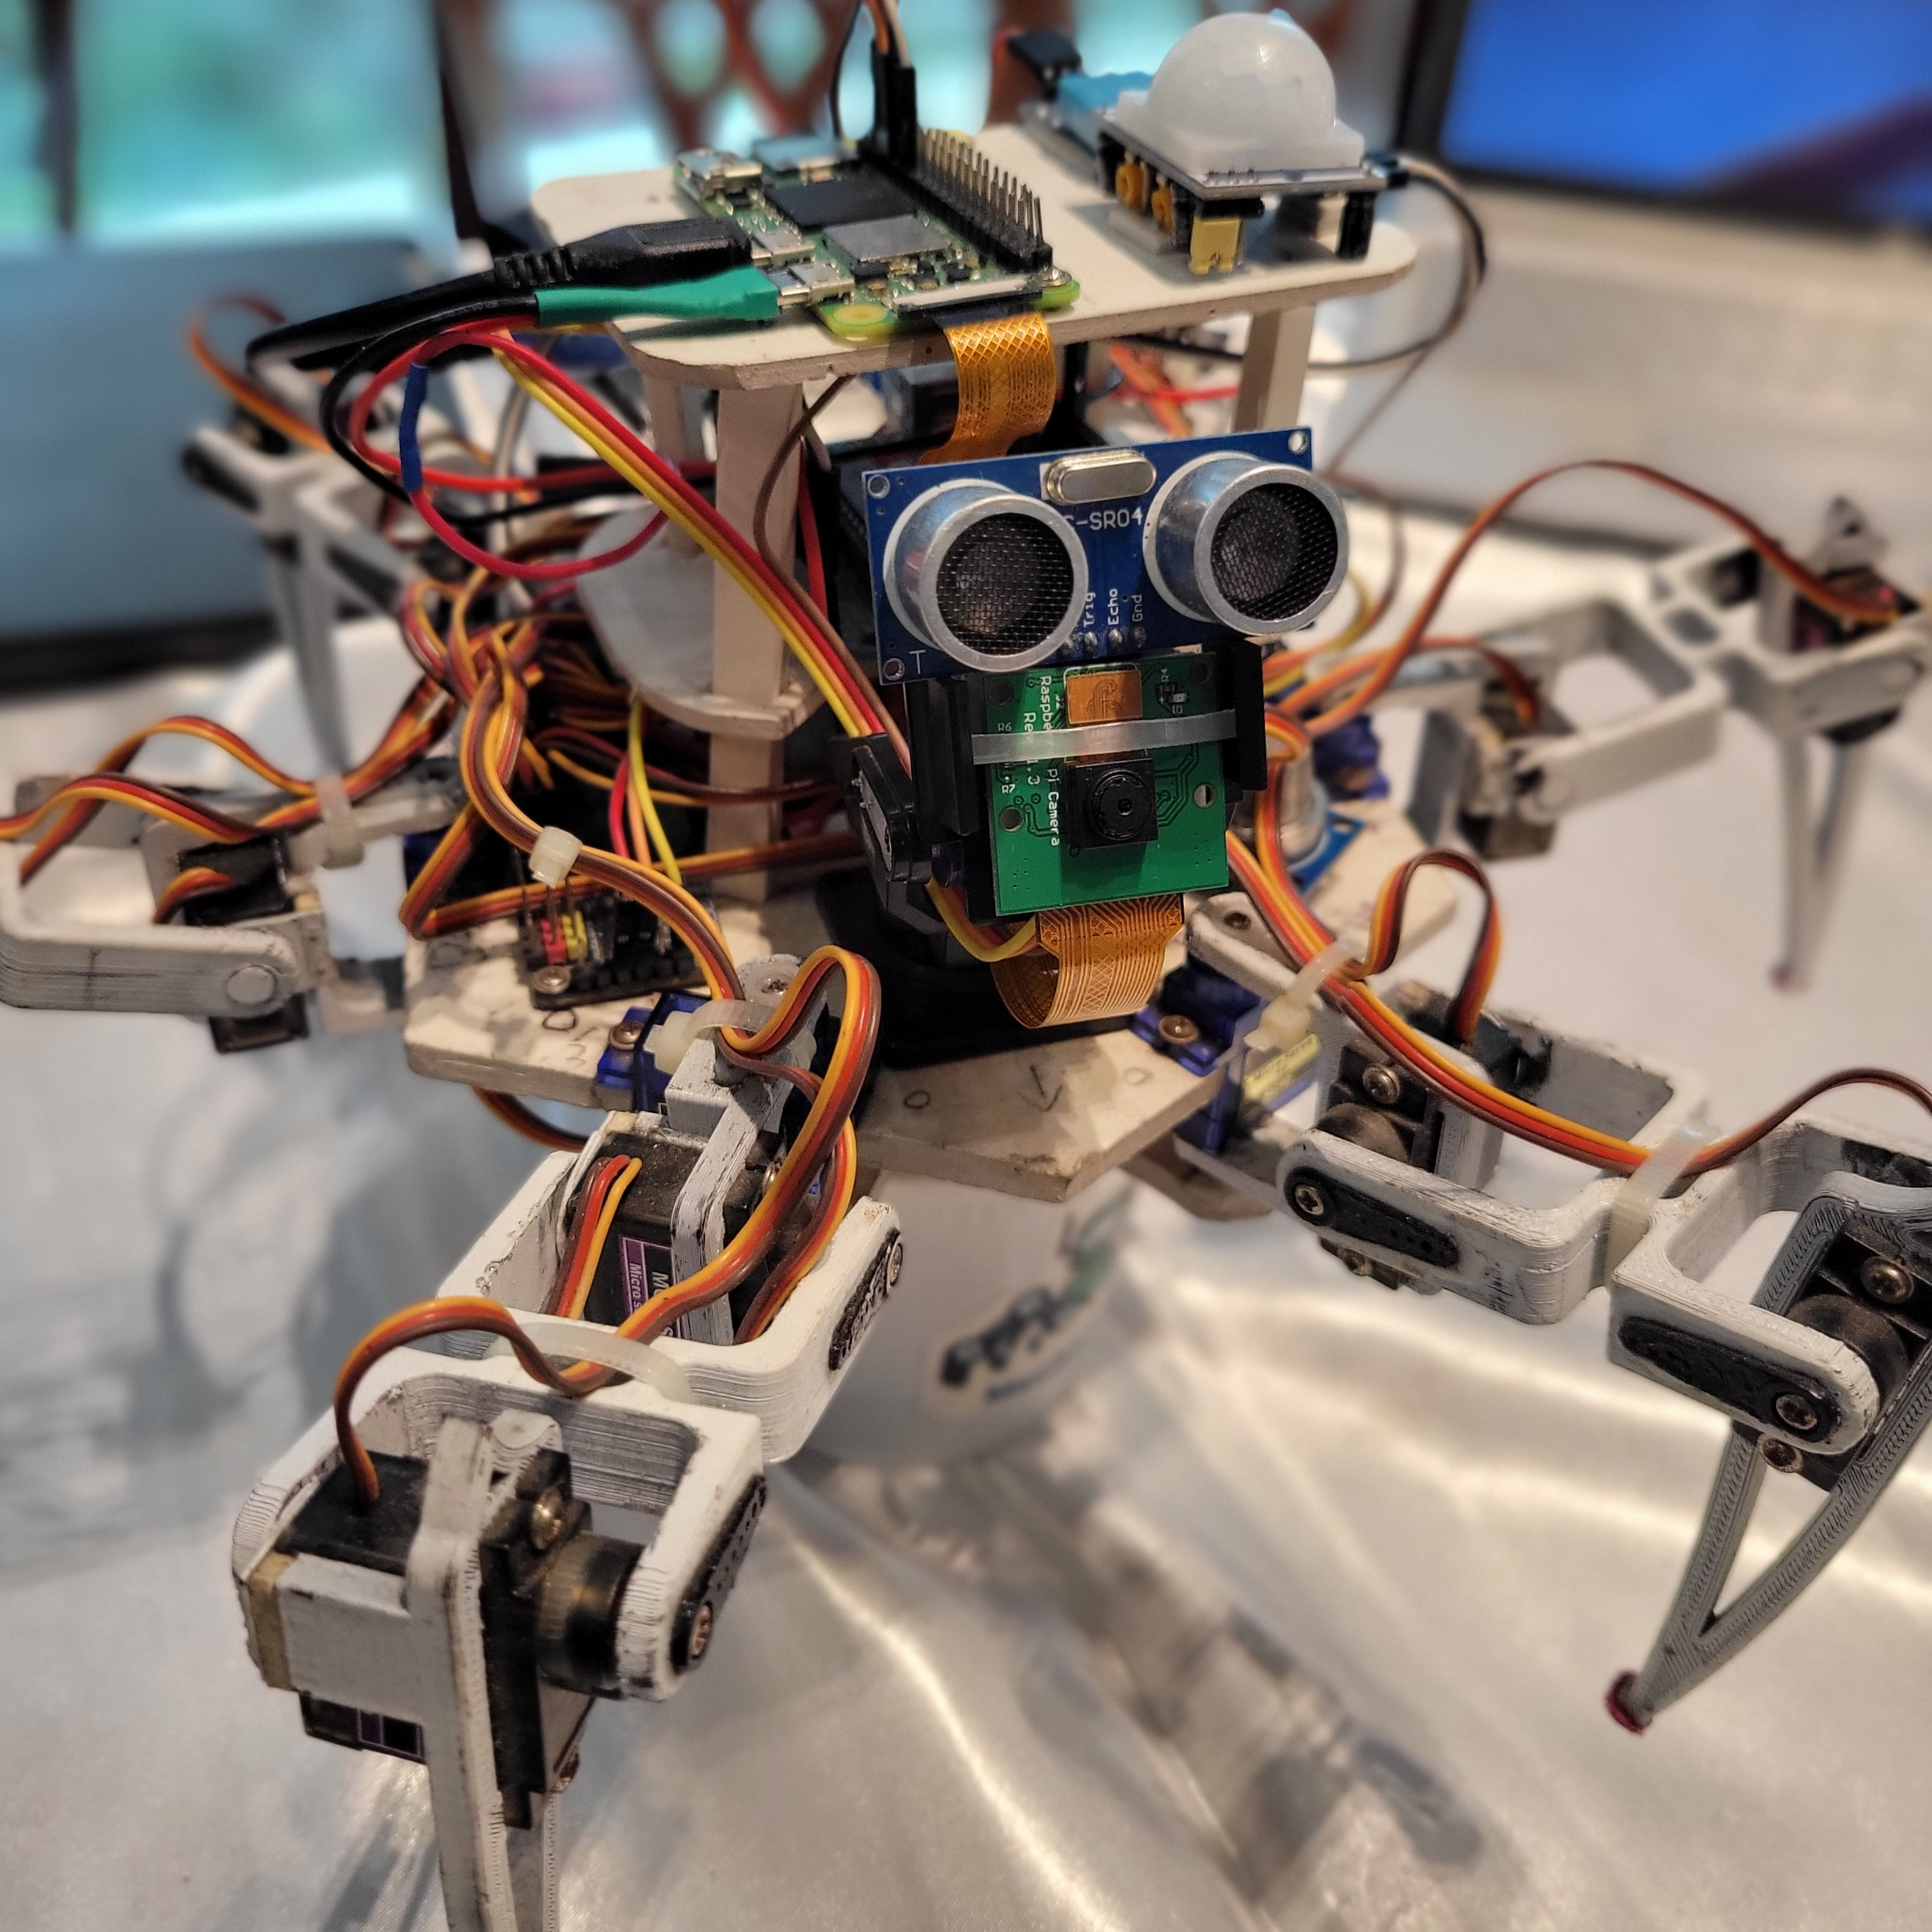
\includegraphics[width=\columnwidth]{walle.jpg}
  \caption*{WALL-E inspired roaming and sensing Robot}
  \label{fig2}
\end{figure}
% Building More section
\section*{You Are Building More Than Projects}
Your community may benefit from something that begins with a blinking light. One day, you might invent a smart farming solution, develop an inexpensive medical device, or motivate young people in your community.

You’re also creating something more significant with every project: your mindset. You’re developing abilities that transcend the classroom: the ability to see issues, envision solutions, and make them a reality.
% Conclusion section
\section*{Conclusion: Start Small, Dream Big}
Don’t wait for the ideal opportunity, funding, or mentor. Start with what you already have. Take lessons from your errors. Tell us about your journey. Robotics is about people like you using basic tools to solve real problems and express their creativity, not just about machines.

So feel free. Tinker. Build. Fail. Give it another go. Take pride. Because creators like you are the ones who will shape the future.\\ \\ \\
Here's a National Robotics Competition arranged by {\href{https://www.facebook.com/BRACU.Robotics.Club?__cft__[0]=AZXasvym4j5qx2lJLvH1OSNuhkeFYoBdxnsV0YdlMU2P3pYb473uPrC4HLQAcX3Ht2_0rOMQPux7ut2yPDebjVkmwSHEyaINIzdgGPzQLzW55ue-jvkM4fqpAYsmdcIPr4kx-rLIVsLGG4Ku40L_JPX5I-TdBlTCh9lwKlUlLzph4A&__tn__=-UC\%2CP-R}{Robotics Club of BRAC University - ROBU}} :  {\href{https://www.facebook.com/BRACU.Robotics.Club/posts/presenting-you-a-sneak-peek-into-%F0%9D%90%93%F0%9D%90%AB%F0%9D%90%9A%F0%9D%90%9C%F0%9D%90%AD%F0%9D%90%A2%F0%9D%90%A8%F0%9D%90%A7-%E0%A6%85%E0%A6%AD%E0%A7%8D%E0%A6%AF%E0%A7%81%E0%A6%A6%E0%A6%AF%E0%A6%BC-the-prestigious-national-robo/1124725119696964/}{Traction}
 
% Side Note Box
\begin{center}
\subsection*{}
\textbf{Curious About Arduino and ESP32?}
\begin{itemize}
    \item Arduino is simple, safe, and beginner-friendly.
    \item ESP32 adds Wi-Fi and Bluetooth, so you can build smart home or IoT devices.
    \item Start with whichever you find—what matters is starting!
\end{itemize}

\end{center}
% Final Spark section
\section*{Final Spark}
Keep a small diary, blog, or social post about each thing you try. A year from now, you’ll look back and smile at how far you’ve come.
\clearpage



%--------------------------------------------------------------------------%
%----------------------------- ARTICLE 7 ----------------------------------%
%--------------------------------------------------------------------------%
\article{\centering{Dopamine: The Currency of Digital Control}}{Md.Asif Khan}

\begin{figure}[h!]
  \centering
  \includegraphics[width=0.9\linewidth]{banana.png}
  \caption*{\textit{A Sweet Struggle: Natural vs. Neurological Reward.}}
\end{figure}

\lettrine[lines=3]{I}{f} 
 we ask a child to pick between a chocolate or a banana, what would it take? In most cases, the answer has to be chocolate. But why? Have we ever thought about it? Is it just because it feels good? Have we ever thought why we sneak into our social media every now and then? Why would we choose to lie in bed with our phone instead of studying at the table? Is it just because it feels good? While that is partially correct, it does not reveal the main reason behind these choices. Our decision-making, addiction, and behavior are all connected to the brain’s reward system, which is controlled by neurotransmitters. Among them, the most common and vital is dopamine.

\section*{What are Neurotransmitters and How Do They Function?}

Neurotransmitters are chemical messengers that transmit signals between brain cells, influencing everything from mood to motivation. Four key neurotransmitters generate pleasure and reward: Dopamine creates motivation and the thrill of anticipation, like when smelling your favorite food cooking. Serotonin provides deep contentment and emotional stability, often boosted by sunlight or meaningful accomplishments. Endorphins act as natural pain relievers that also induce euphoria, such as the 'runner's high' after intense exercise. Oxytocin promotes bonding and warmth, released during hugs or moments of trust. Together, these chemicals shape life's most rewarding experiences.

\section*{The Role of Dopamine as a Neurotransmitter}

Dopamine is a neurotransmitter—or brain chemical—that people sometimes call the "feel good" hormone. That's because when we do things that trigger the release of dopamine, we feel good. In fact, we sometimes feel so good that we seek out those experiences over and over again. We discussed a child’s choice of chocolate over a banana. We said it is because it feels good. But how is dopamine related to this?

Actually, when we perceive things, our brain scans every bit of information and calculates which option would give us maximum reward. But the question is, what’s a reward? A reward is anything our brain sees as good. It could be something small, like a smile or something big, like winning a trophy. Dopamine helps our brain remember rewards! Dopamine plays a big role when we make choices. It helps our brain decide if something is worth doing. It helps us weigh the rewards and the risks. Every time we think about doing something fun, risky, or new, dopamine is part of that decision. Similarly, when a child is asked to decide between chocolate and a banana, their brain analyzes the two and picks chocolate as more rewarding or more dopamine-releasing. That’s how dopamine influences our decisions.

\section*{Social Media’s UI/UX and Algorithms}

In today’s digital age, social media platforms have become an integral part of our daily lives, offering instant connectivity, entertainment, and information at our fingertips. However, beneath the surface of these seemingly harmless interactions lies a complex interplay between our brain’s chemistry and the carefully designed features of social media apps. Features like likes, comments, shares, stories, and reels often compel us to stick to social media for a long time.

\begin{figure}[h!]
  \centering
  \includegraphics[width=0.9\linewidth]{brended.png}
  \caption*{\textit{Swipe, Scroll, Reward: The Brain Loves a Good Notification}}
\end{figure}

Have we ever thought about why there’s no end to newsfeed scrolling or reel watching? The continuous notifications or pull-to-refresh features make us spend a long time on social media. Sometimes, we pick up our phone just because of a notification sound from social media, only to end up wasting an hour for no real reason. These platforms are designed to trigger dopamine release, creating a rewarding cycle that keeps users coming back for more. The brain’s reward system responds to likes, comments, and shares, releasing small bursts of dopamine with each interaction. This neurochemical response reinforces the behavior, making social media use habit-forming and potentially addictive. These features also cause FOMO (fear of missing out), which leads teens to get addicted to social media influence and reach.

One of the most concerning aspects is the algorithm that serves us our preferred content. Ever wondered how social media knows what your favorite content is and which contents tend to keep you long time on screen? You might discuss the "Final Destination" movie with friends, and the next day your Instagram reels are filled with related content. Or you text a friend about needing an ESP32 microcontroller for a project, and suddenly you see ads for it everywhere.

How do they know what you need? The answer is simple: we give permissions like location, voice, and camera to the social media app. Using all those permissions, they analyze our personal data along with our posts or interaction data through artificial intelligence. Then they display specific content or items. Once I stared at a person’s story for a few seconds, and then Facebook started to show that person’s posts and stories at the top of my feed. That’s how their algorithms function—to keep us on their apps for as long as possible.

\section*{Breaking the Habit}

Breaking the cycle of social media addiction begins with awareness. Setting boundaries, such as limiting screen time, turning off non-essential notifications, and creating tech-free zones, can help reduce compulsive use. Practicing mindfulness, pausing to ask why you are reaching for your phone can help you regain control.
\begin{figure}[h!]
  \centering
  \includegraphics[width=0.9\linewidth]{pop.png}
  \caption*{\textit{Neuro-freedom: Real Life > Notifications.}}
\end{figure}
Engaging in activities that naturally boost dopamine, such as exercise, creative hobbies, or spending time with friends and family can provide healthier sources of reward. Understanding how social media is designed to capture your attention empowers you to make more intentional choices about your digital habits. With conscious effort, it is possible to reclaim your time and attention from the grip of digital dopamine triggers.

\section*{References}

\begin{enumerate}
    \item Volkow, N. D., \& Morales, M. (2015). The Brain on Drugs: From Reward to Addiction. \href{https://www.cell.com/neuron/pdf/S0896-6273(15)00133-6.pdf}{PDF Link}
    \item Webmedy. Dopamine and Decision Making. \href{https://webmedy.com/blog/dopamine-decision-making/}{https://webmedy.com/blog/dopamine-decision-making/}
    \item OurMental.Health. Hooked on Dopamine. \href{https://www.ourmental.health/screen-time-sanity/hooked-on-dopamine-how-social-media-hijacks-your-brain}{https://www.ourmental.health/...}
    \item Neurolaunch. Social Media and Dopamine. \href{https://neurolaunch.com/social-media-dopamine/}{https://neurolaunch.com/social-media-dopamine/}
    \item Glass Almanac. How Dopamine Influences Behavior and Decision-Making According to Science. \href{https://glassalmanac.com/how-dopamine-influences-behavior-and-decision-making-according-to-science/}{https://glassalmanac.com/...}
    \item Healthline. Dopamine Addiction. \href{https://www.healthline.com/health/dopamine-addiction}{https://www.healthline.com/health/dopamine-addiction}
    \item Verywell Mind. Can You Get Addicted to Dopamine? \href{https://www.verywellmind.com/can-you-get-addicted-to-dopamine-5207433}{https://www.verywellmind.com/...}
\end{enumerate} 

\clearpage


%--------------------------------------------------------------------------%
%----------------------------- ARTICLE 8 ----------------------------------%
%--------------------------------------------------------------------------%

\article{\centering{The Silent Revolution}}{Muhaimin Kamran}{}
\begin{figure}[h!]
  \centering
  \includegraphics[width=0.6\linewidth]{brainchip.png}
  \caption*{\textit{Visual depiction of a brain-computer interface enabling control through thought—a breakthrough achieved by Neuralink’s first human trials.}}
\end{figure}
\lettrine[lines=3]{O}{nce} \textbf{science fictions} were dismissed as mere fantasy. In 1864, \textbf{Jules Verne} wrote \textit{Journey to the Center of the Earth}, where he described a mission to the Moon—launched from Florida. Then, in 1870, he penned \textit{20,000 Leagues Under the Sea}, in which \textbf{Captain Nemo} traveled beneath the ocean in an electric-powered submarine. Decades later, in 1969, \textbf{Neil Armstrong} stepped onto the Moon during the Apollo 11 mission—and science fiction began turning into reality. Today, detailed underwater exploration is routine. \textbf{Sci-fi started becoming real}.

In January 2024, the first successful \textbf{brain-computer interface (BCI)} was implanted—a tiny device in the brain allowing humans to interact directly with computers, AI, or prosthetics. \textbf{Noland Arbaugh}, a young man left quadriplegic after a diving accident, became the first human subject. \textbf{Neuralink} implanted a chip—called the \textbf{“Link”}—into the region of his brain that controls movement. The chip has sixty-four threads, each thinner than human hair, placed precisely by a \textbf{surgical robot}. With it, Noland can move a computer mouse using only his thoughts. He now browses the internet, plays chess, and navigates online tools without moving a single muscle. Neuralink even livestreamed him playing chess on a MacBook using only brain signals. By mid-June 2025, \textbf{BCI’s initial implementation had proven successful}. \textbf{dshufliaf}. 

Meanwhile, AI systems, especially those developed by \textbf{OpenAI} and others—have performed remarkably well in standardized exams designed for humans. For example, AI passed all three steps of the \textbf{USMLE} (medical licensing exam), scored in the \textbf{top 10\%} on the \textbf{Bar Exam}, and placed around the 90th percentile on the \textbf{LSAT} (law school admission test). It scored between 1400 and 1550 on the \textbf{SAT} and performed at around the 99th percentile in verbal reasoning and 85th percentile in quantitative reasoning on the \textbf{GRE}. On \textbf{AP exams}, AI typically scores \textbf{4s and 5s}. On top of that, it solves coding challenges across platforms like \textbf{LeetCode} and in competitive programming environments.

AI has also discovered \textbf{Halicin}—a novel antibiotic—by exploring chemical spaces that no human ever had. \textbf{DeepMind’s AlphaFold} predicted the 3D structure of nearly every known protein. AI can now generate full software apps, websites, scripts, even games—just from a prompt. AI tools produce short films, stunning artwork, and realistic human faces that don’t exist. \textbf{DeepMind’s AlphaStar} has beaten \textbf{99.8\%} of all human \textit{StarCraft II} players.

We once dreamed of the future. \textbf{Now, the future has awakened—before we were ready}.

In the coming years, we may see \textbf{mass adoption of BCIs}. Human thinking, analysis, and imagination could begin to merge with real-time internet data. It may even become possible for someone to \textbf{spy on our thoughts}.

\textbf{AI-powered robo-doctors} or \textbf{AI judges} may become mainstream—cost-effective, efficient, and widely accessible. At the same time, AI capable of exploring chemical spaces might design \textbf{deadly pathogens}. Automated law enforcement systems could operate with no empathy or human oversight. Governments may use legal AI to justify censorship or oppression. Fake videos, false news, and synthetic war footage will become harder to detect. Identities may be lost, as AI perfectly mimics faces, voices, and writing styles.

\begin{figure}[h!]
  \centering
  \includegraphics[width=0.6\linewidth]{aivlona.png}
  \caption*{\textit{As AI grows more powerful, the line between empowerment and manipulation blurs. Regulation is essential to preserve identity and ethics in the age of algorithms.}}
\end{figure}

\textbf{These technologies are advancing faster than the laws that govern them.} If left unchecked, tools designed to empower humanity could destabilize it. Regulation does not mean halting progress, it means steering it toward safe, fair outcomes.

\textbf{We are not yet at the point where AI thinks independently, like in science fiction.} But we are moving faster than we ever imagined. The convergence of AI, brain interfaces, and quantum computing marks a profound turning point in human history.

These tools carry tremendous promise—cures for diseases, universal access to knowledge, freedom from disability, and global efficiency. But without thoughtful regulation, rigorous testing, and transparent governance, they may also introduce risks for which we are not yet prepared. \textbf{We do not fear the future; we fear that it is already here}.
\clearpage


% ====================
% Epilogue
% ====================
\clearpage
\onecolumn
\section*{Epilogue}
\addcontentsline{toc}{section}{Epilogue}
\vspace*{0.2cm}
As we close this inaugural issue of \textit{The Aevum}, we reflect on the collective effort that brought these ideas to life. This magazine represents more than just articles—it's a testament to curiosity, collaboration, and the courage to explore complex questions.

\vspace{0.4em}
\begin{center}
\textbf{Contributors:}
\end{center}
\begin{multicols}{2}
% Left column: First 3 contributors
\begin{itemize}[leftmargin=*, label={}]
  \item \contributor{Maliha Laheen}{322}{20240659104}{Editor}
  \item \contributor{Ferdous Ara Fahima}{323}{20240659105}{Proofreader}
  \item \contributor{Sultana Akter}{325}{20240659107}{Reviewer}
\end{itemize}
\columnbreak
% Right column: Next 4 contributors
\begin{itemize}[leftmargin=*, label={}]
  \item \contributor{Md. Asif Khan}{348}{20240659130}{Typesetter}
  \item \contributor{Md. Kaif Ibn Zaman}{358}{20240659140}{Reviewer}
  \item \contributor{Muhaimin Kamran}{366}{20240659148}{Typesetter}
  \item \contributor{Tamjeed Rahman Udoy}{373}{20240659155}{Proofreader}
\end{itemize}
\end{multicols}

% Group Photo
\begin{figure}[H]
  \centering
  \includegraphics[width=0.6\textwidth]{group_photo.jpg}
  \caption*{The creative team behind \textit{The Aevum}}
\end{figure}

\vspace{0.4em}
\begin{center}
{\small\scshape\color{gray}Until next time, stay curious.}
\end{center}
\cleardoublepage
\twocolumn



% ====================
% BACK PAGE
% ====================
\cleardoublepage % Clear content from contributors page
\thispagestyle{empty}
\AddToShipoutPictureBG*{%
  \AtPageLowerLeft{%
    \includegraphics[width=\paperwidth, height=\paperheight]{BACK_cover.png}
  }
}
\null % Ensure the page is fully occupied
% \cleardoublepage % Ensure no content follows
\end{document}
